\documentclass[10pt,aspectratio=169]{beamer}

\usepackage[T1]{fontenc}
\usepackage[utf8]{inputenc}
\usepackage{lmodern}
\usepackage{graphicx}
\usepackage{booktabs}
\usepackage{adjustbox}
\usepackage{amsmath}

\setbeamertemplate{navigation symbols}{}
\setbeamertemplate{headline}{}
\setbeamertemplate{footline}{%
  \hfill\raisebox{0.6em}{\scriptsize\insertframenumber/\inserttotalframenumber}\hspace{1em}}
\setbeamertemplate{frametitle}{%
  \vspace{0.35em}\insertframetitle\par\vspace{0.25em}}
\setbeamercolor{normal text}{fg=black,bg=white}
\setbeamercolor{background canvas}{bg=white}
\setbeamercolor{frametitle}{fg=black,bg=white}
\setbeamercolor{title}{fg=black}
\setbeamercolor{subtitle}{fg=black}
\setbeamercolor{author}{fg=black}
\setbeamercolor{institute}{fg=black}
\setbeamercolor{itemize item}{fg=black}
\setbeamercolor{itemize subitem}{fg=black}
\setbeamerfont{frametitle}{size=\Large,series=\bfseries}
\setbeamerfont{title}{size=\LARGE,series=\bfseries}

\newcommand{\source}[1]{\par\vspace{0.2em}{\scriptsize\color{gray}Source: #1}}

\title{Inflation Inequality Across the Euro Area}
\author{Erwan Gautier \and J\'er\'emi Montorn\`es}
\institute{Banque de France}
\date{}

\begin{document}

% 1
\begin{frame}[plain]
  \centering
  \vspace{0.20\textheight}
  {\LARGE\bfseries Inflation Inequality Across the Euro Area\par}
  \vspace{1.2em}
  {\large Erwan Gautier \qquad J\'er\'emi Montorn\`es\par}
  \vspace{0.6em}
  {\normalsize Banque de France\par}
\end{frame}

% 2
\begin{frame}{Motivation, Research Question, and Literature}
\begin{itemize}
  \item Central banks target aggregate inflation, but households consume different baskets.
  \item The 2021--2023 episode combined high aggregate inflation with large relative-price shocks in energy and food.
  \item How different was inflation across income, age, and residence groups in the euro area?
  \item Which products and production-network channels generated these differences?
  \item Did household price policies reduce average inflation and inflation inequality?
  \item The paper connects research on household-specific inflation, distributional inflation channels, energy exposure, and unconventional fiscal policy.
  \item Related work includes Doepke and Schneider; Kaplan and Schulhofer-Wohl; Jaravel; Pallotti et al.; Claeys et al.; Levell et al.; and Gautier et al.
\end{itemize}
\end{frame}

% 3
\begin{frame}{Data and Methodology}
\begin{itemize}
  \item Monthly Eurostat HICP price indices and item weights, harmonized across euro-area countries.
  \item Aggregate HBS tabulations provide expenditure shares by income, age, residence, and COICOP category.
  \item Individual HBS microdata provide household expenditures, disposable income, demographics, and survey weights.
  \item HBS expenditures are harmonized with HICP items through a COICOP bridge.
  \item Group-specific expenditure weights are estimated using RAS balancing.
  \item Country-level chained Laspeyres indices are aggregated using annual HICP country weights.
\end{itemize}
\[
P_{g,t}=P_{g,t-1}\sum_k w_{gk,t-1}\frac{p_{k,t}}{p_{k,t-1}},
\qquad
\pi_{g,t}=100\left(\frac{P_{g,t}}{P_{g,t-12}}-1\right).
\]
\end{frame}

% 4
\begin{frame}{Short-Run Inflation Inequality by Income Quintile}
\centering
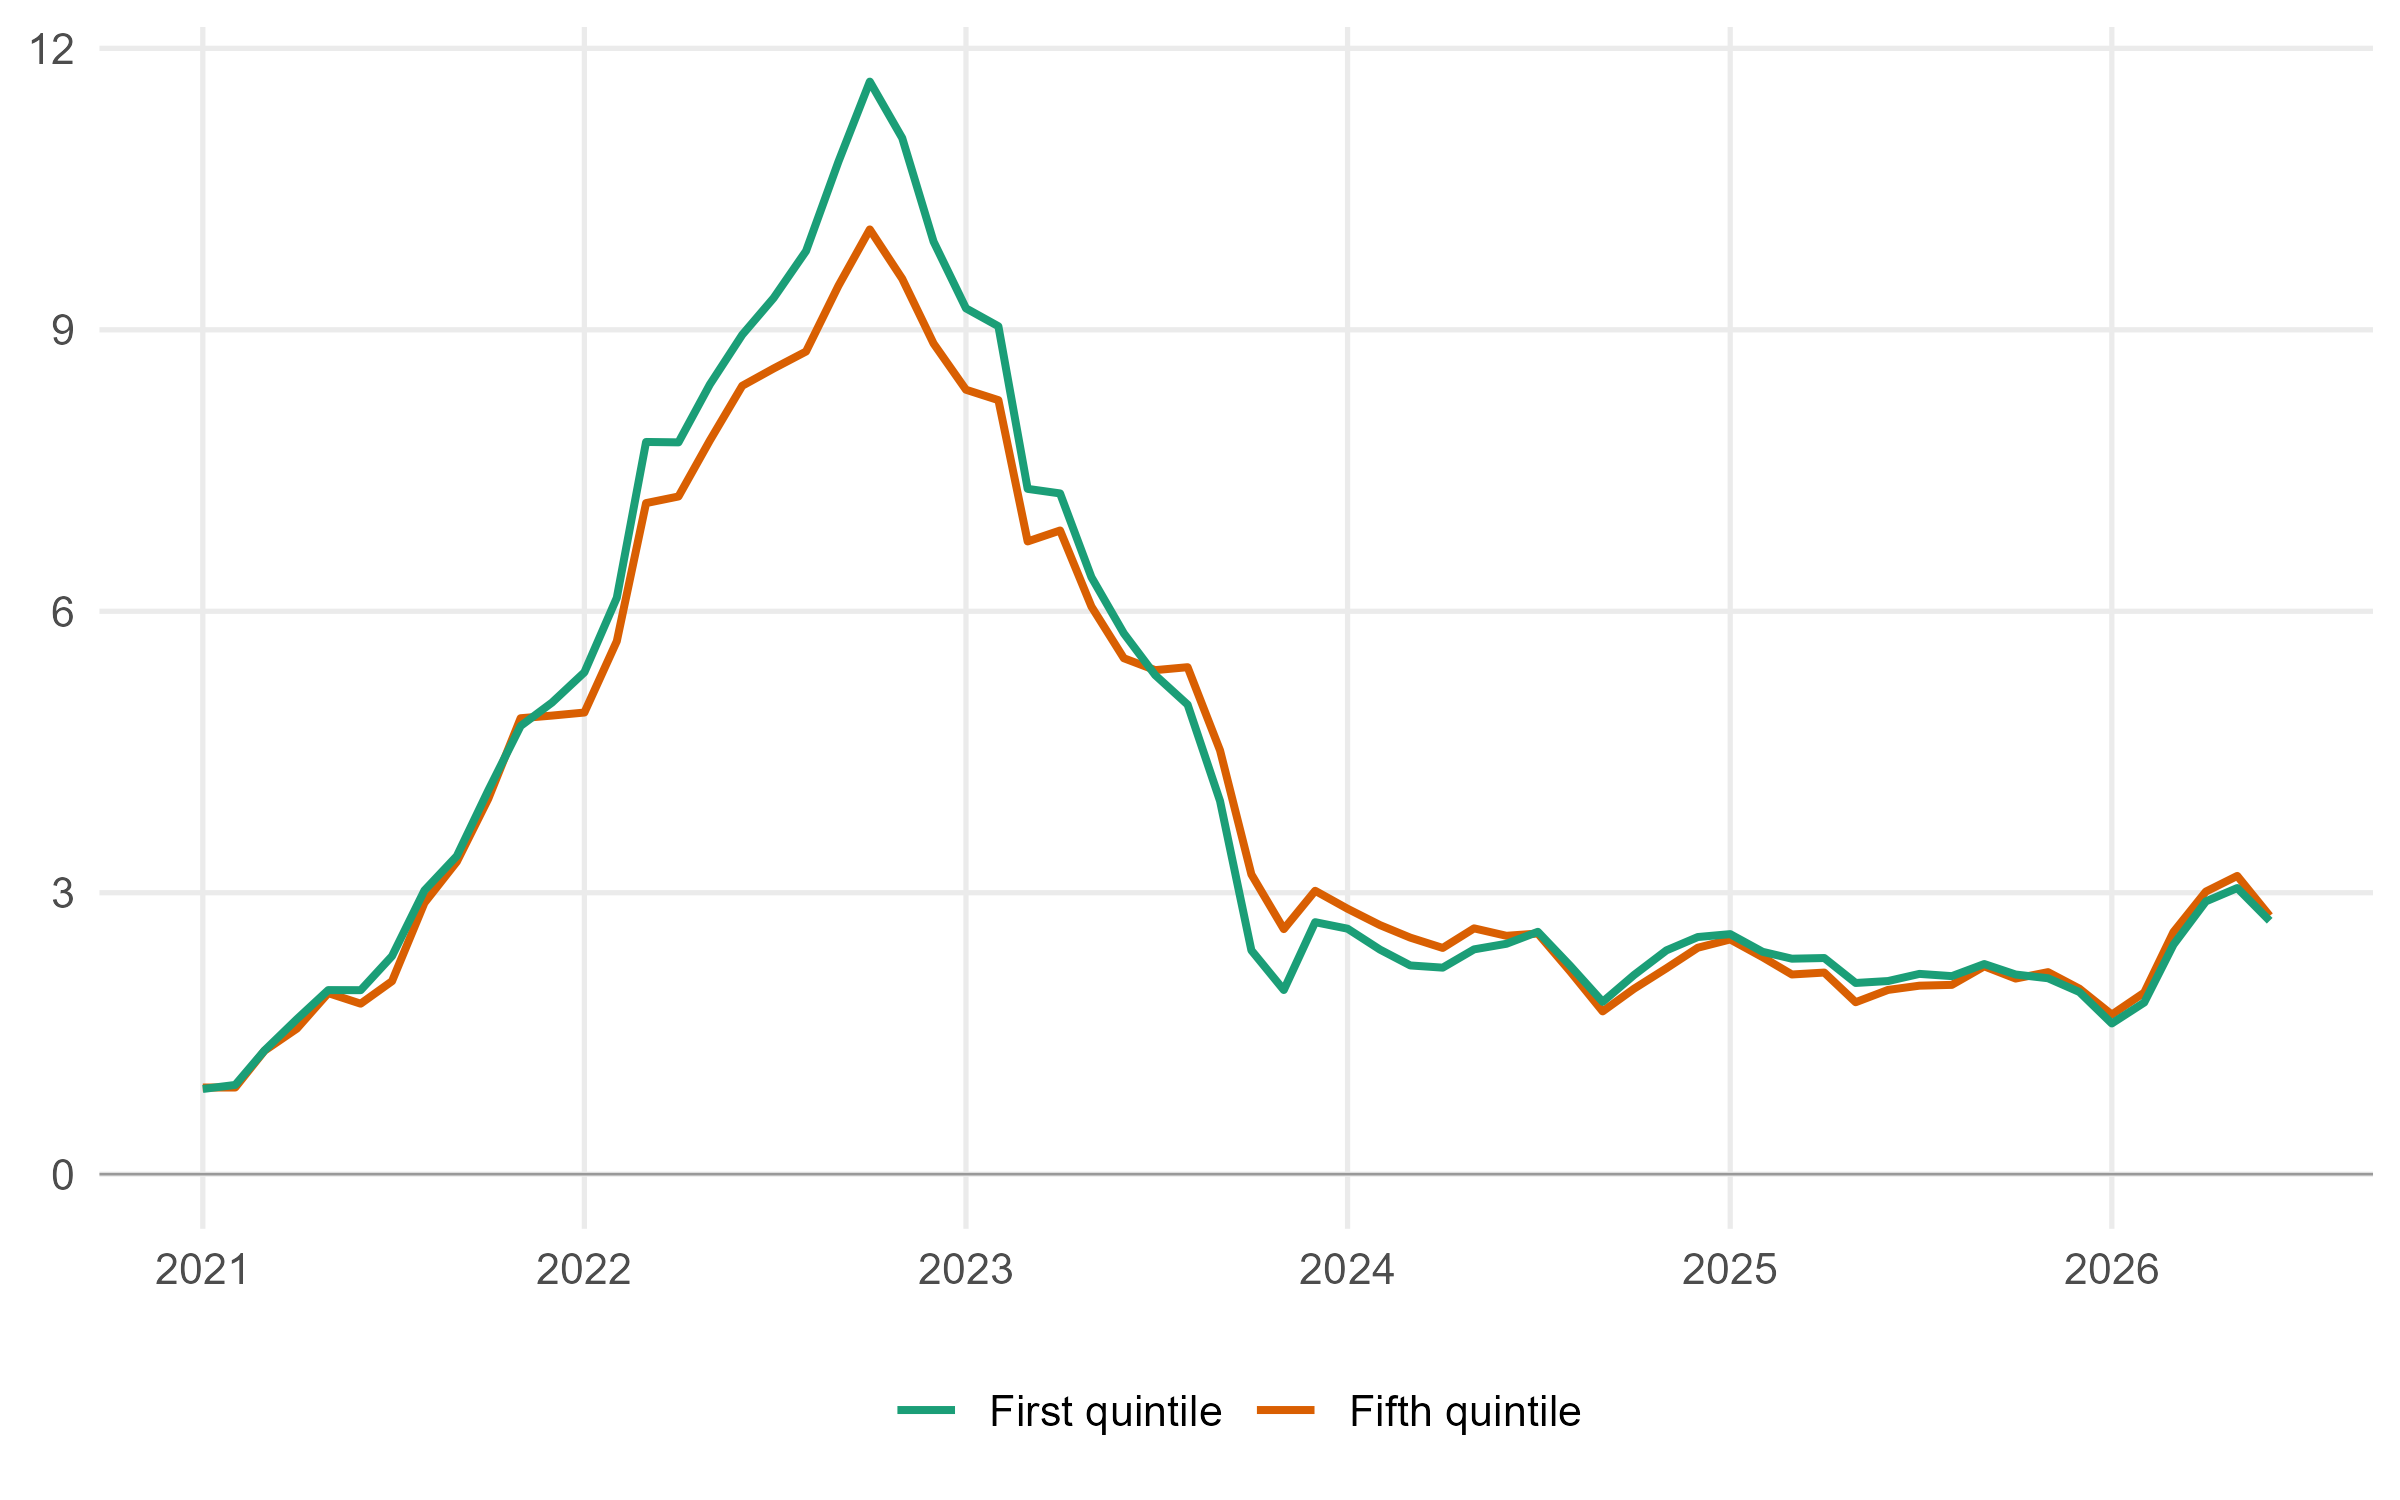
\includegraphics[width=0.82\textwidth,height=0.70\textheight,keepaspectratio]{fig/fig_EA20_2020_2026_income_inflation_Q1_Q5.png}
\source{Eurostat HICP and HBS; authors' calculations.}
\end{frame}

% 5
\begin{frame}{Inflation Inequality by Age}
\centering
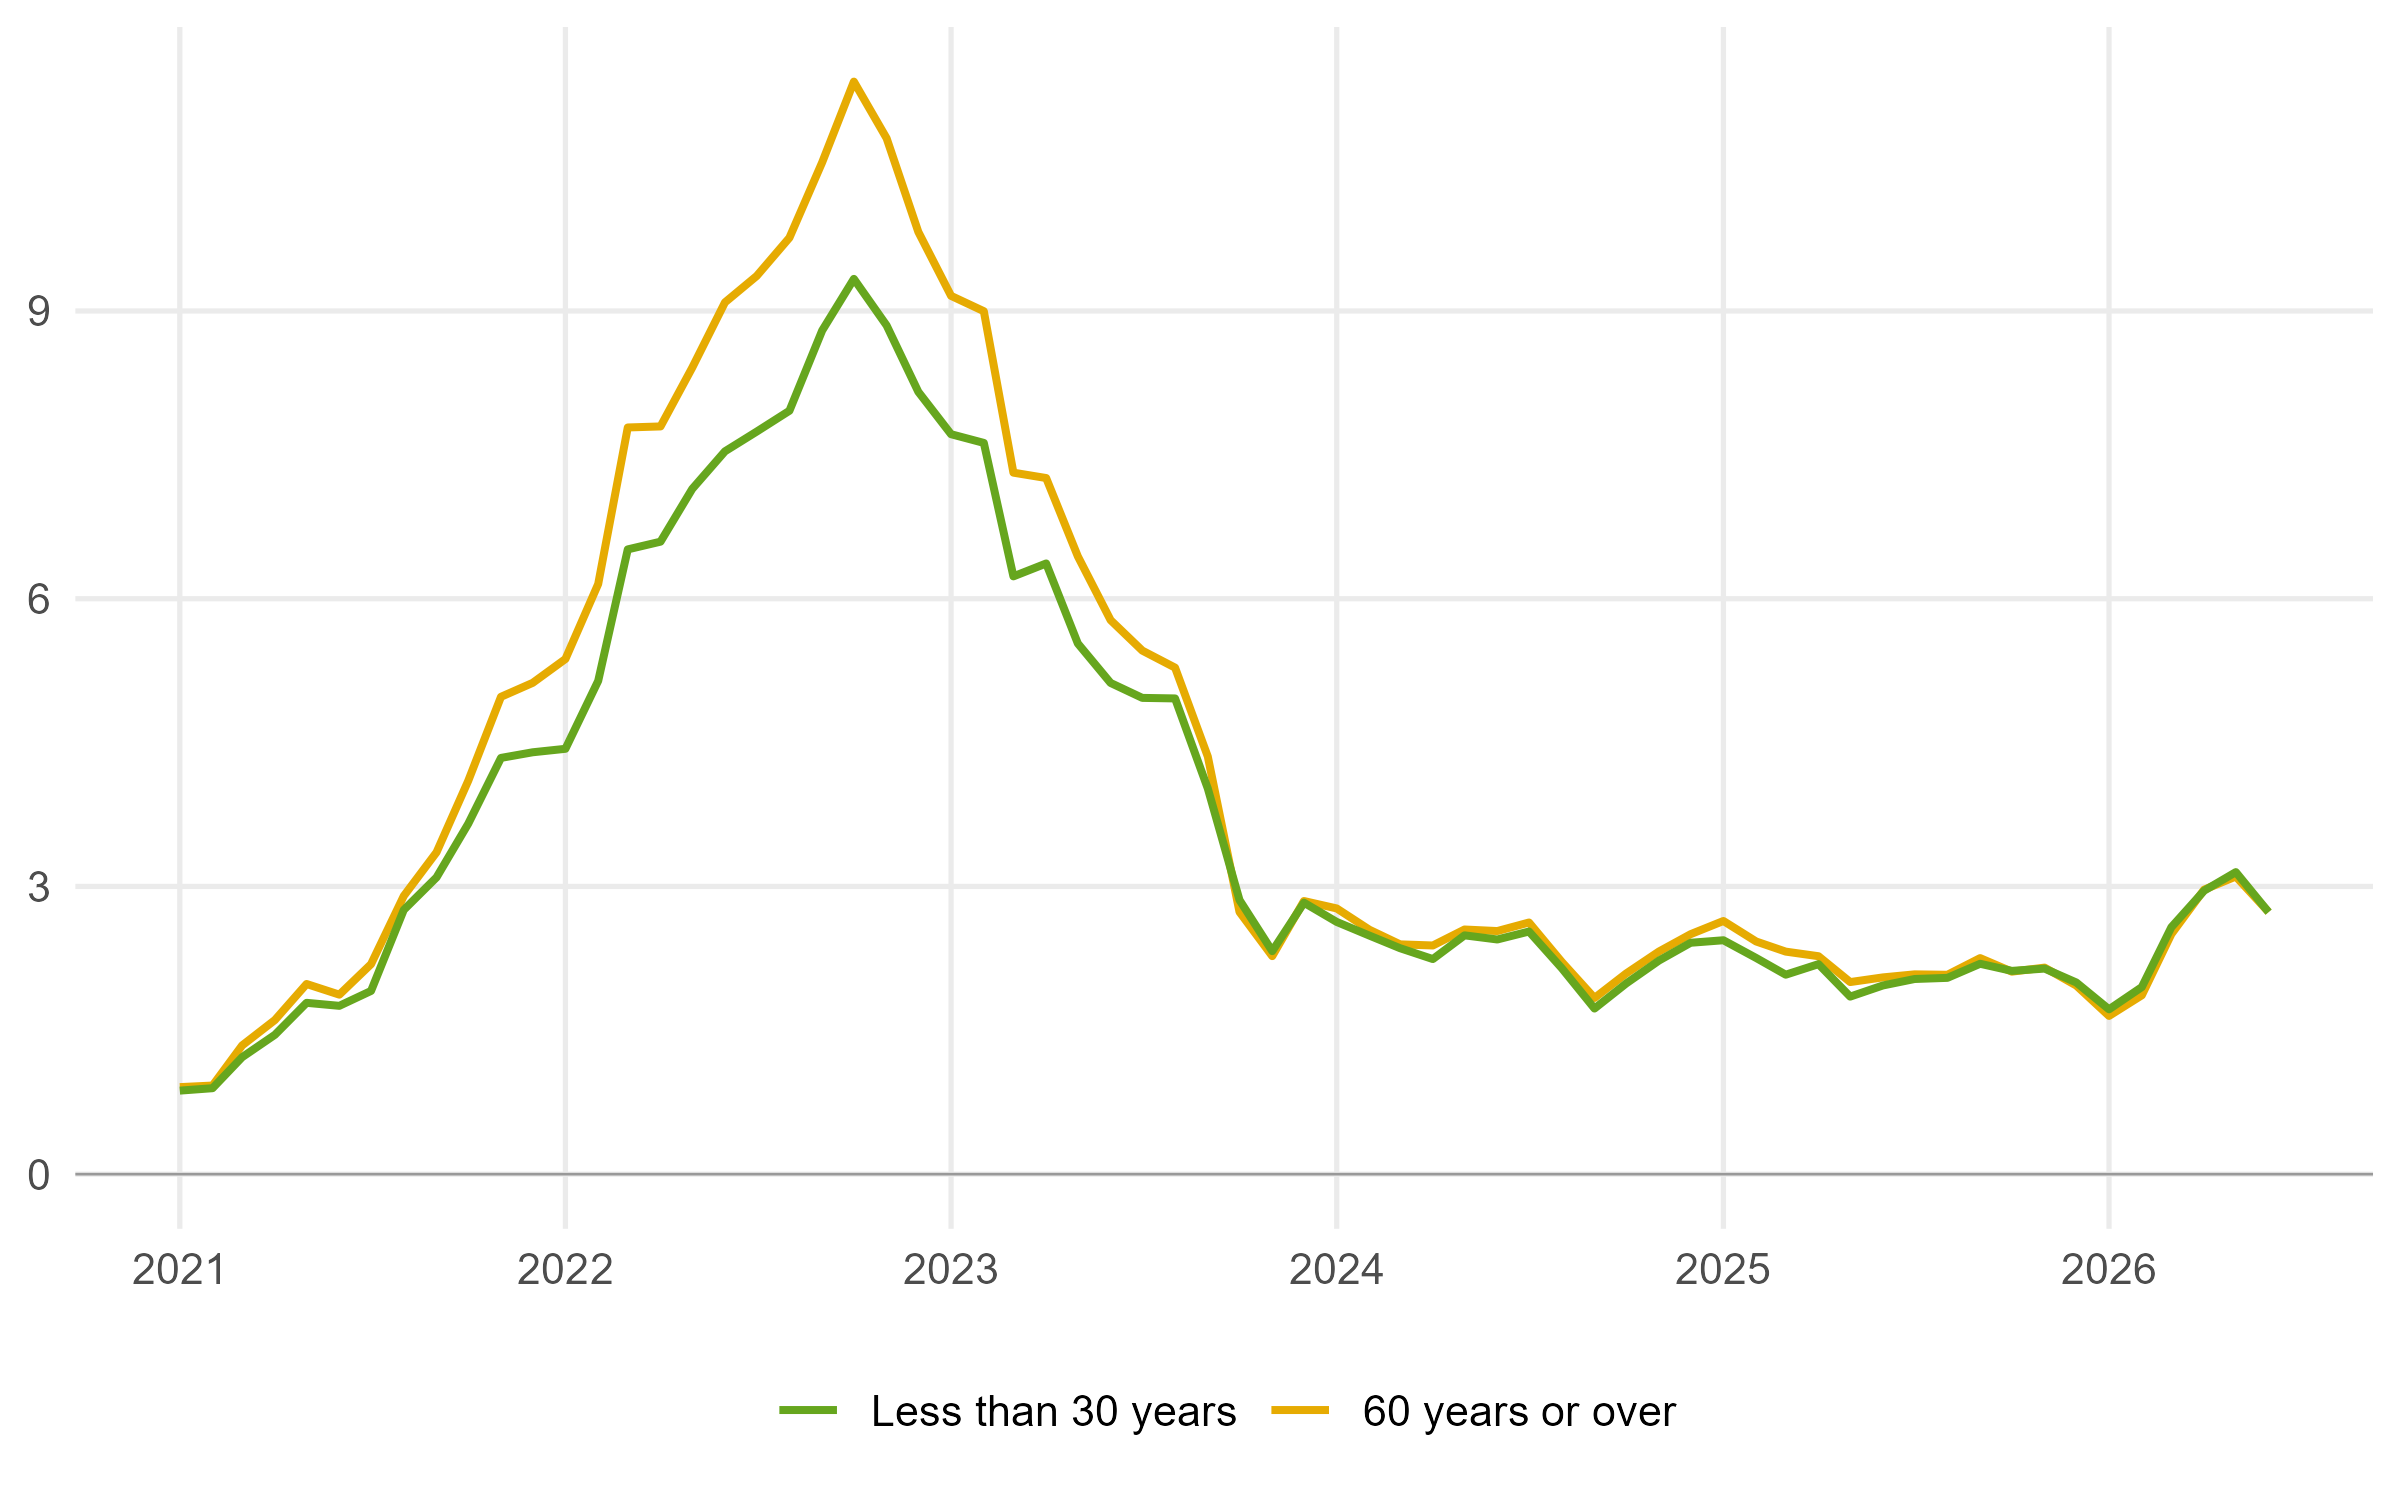
\includegraphics[width=0.82\textwidth,height=0.70\textheight,keepaspectratio]{fig/fig_EA20_2020_2026_age_inflation_under30_60plus.png}
\source{Eurostat HICP and HBS; authors' calculations.}
\end{frame}

% 6
\begin{frame}{Inflation Inequality by Residence Area}
\centering
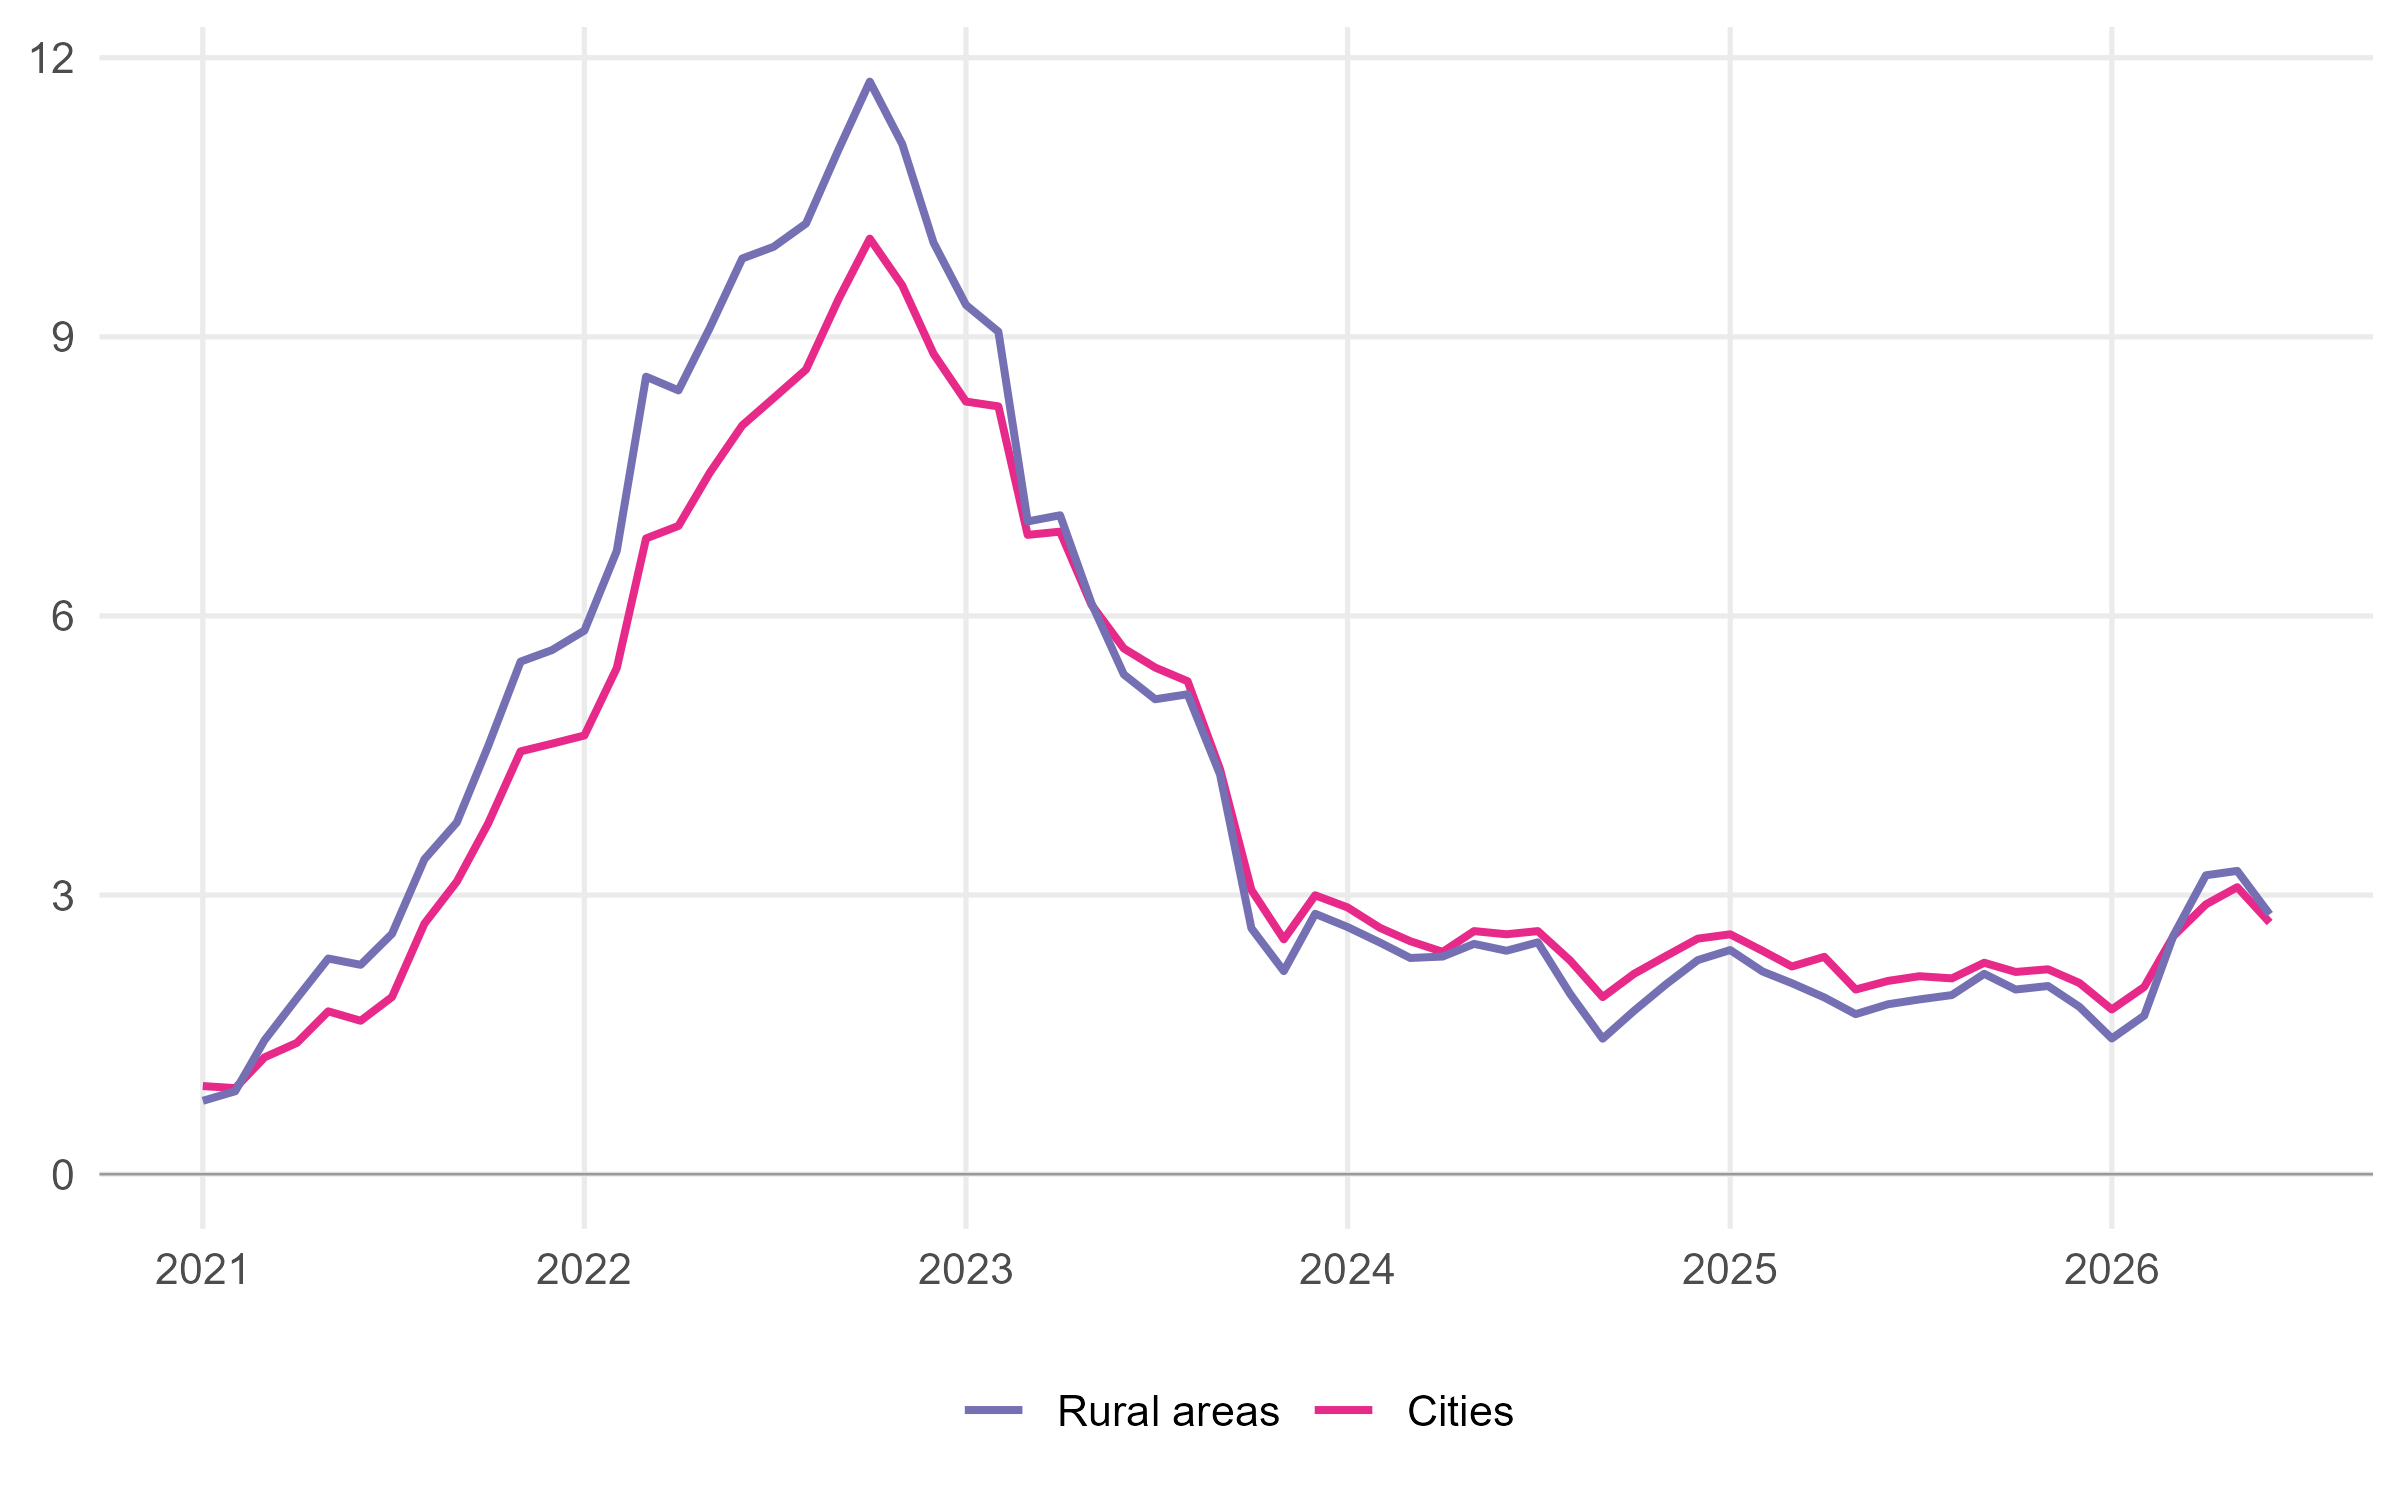
\includegraphics[width=0.82\textwidth,height=0.70\textheight,keepaspectratio]{fig/fig_EA20_2020_2026_urban_inflation_rural_cities.png}
\source{Eurostat HICP and HBS; authors' calculations.}
\end{frame}

% 7
\begin{frame}{Long-Run Inflation Inequality by Income Quintile}
\centering
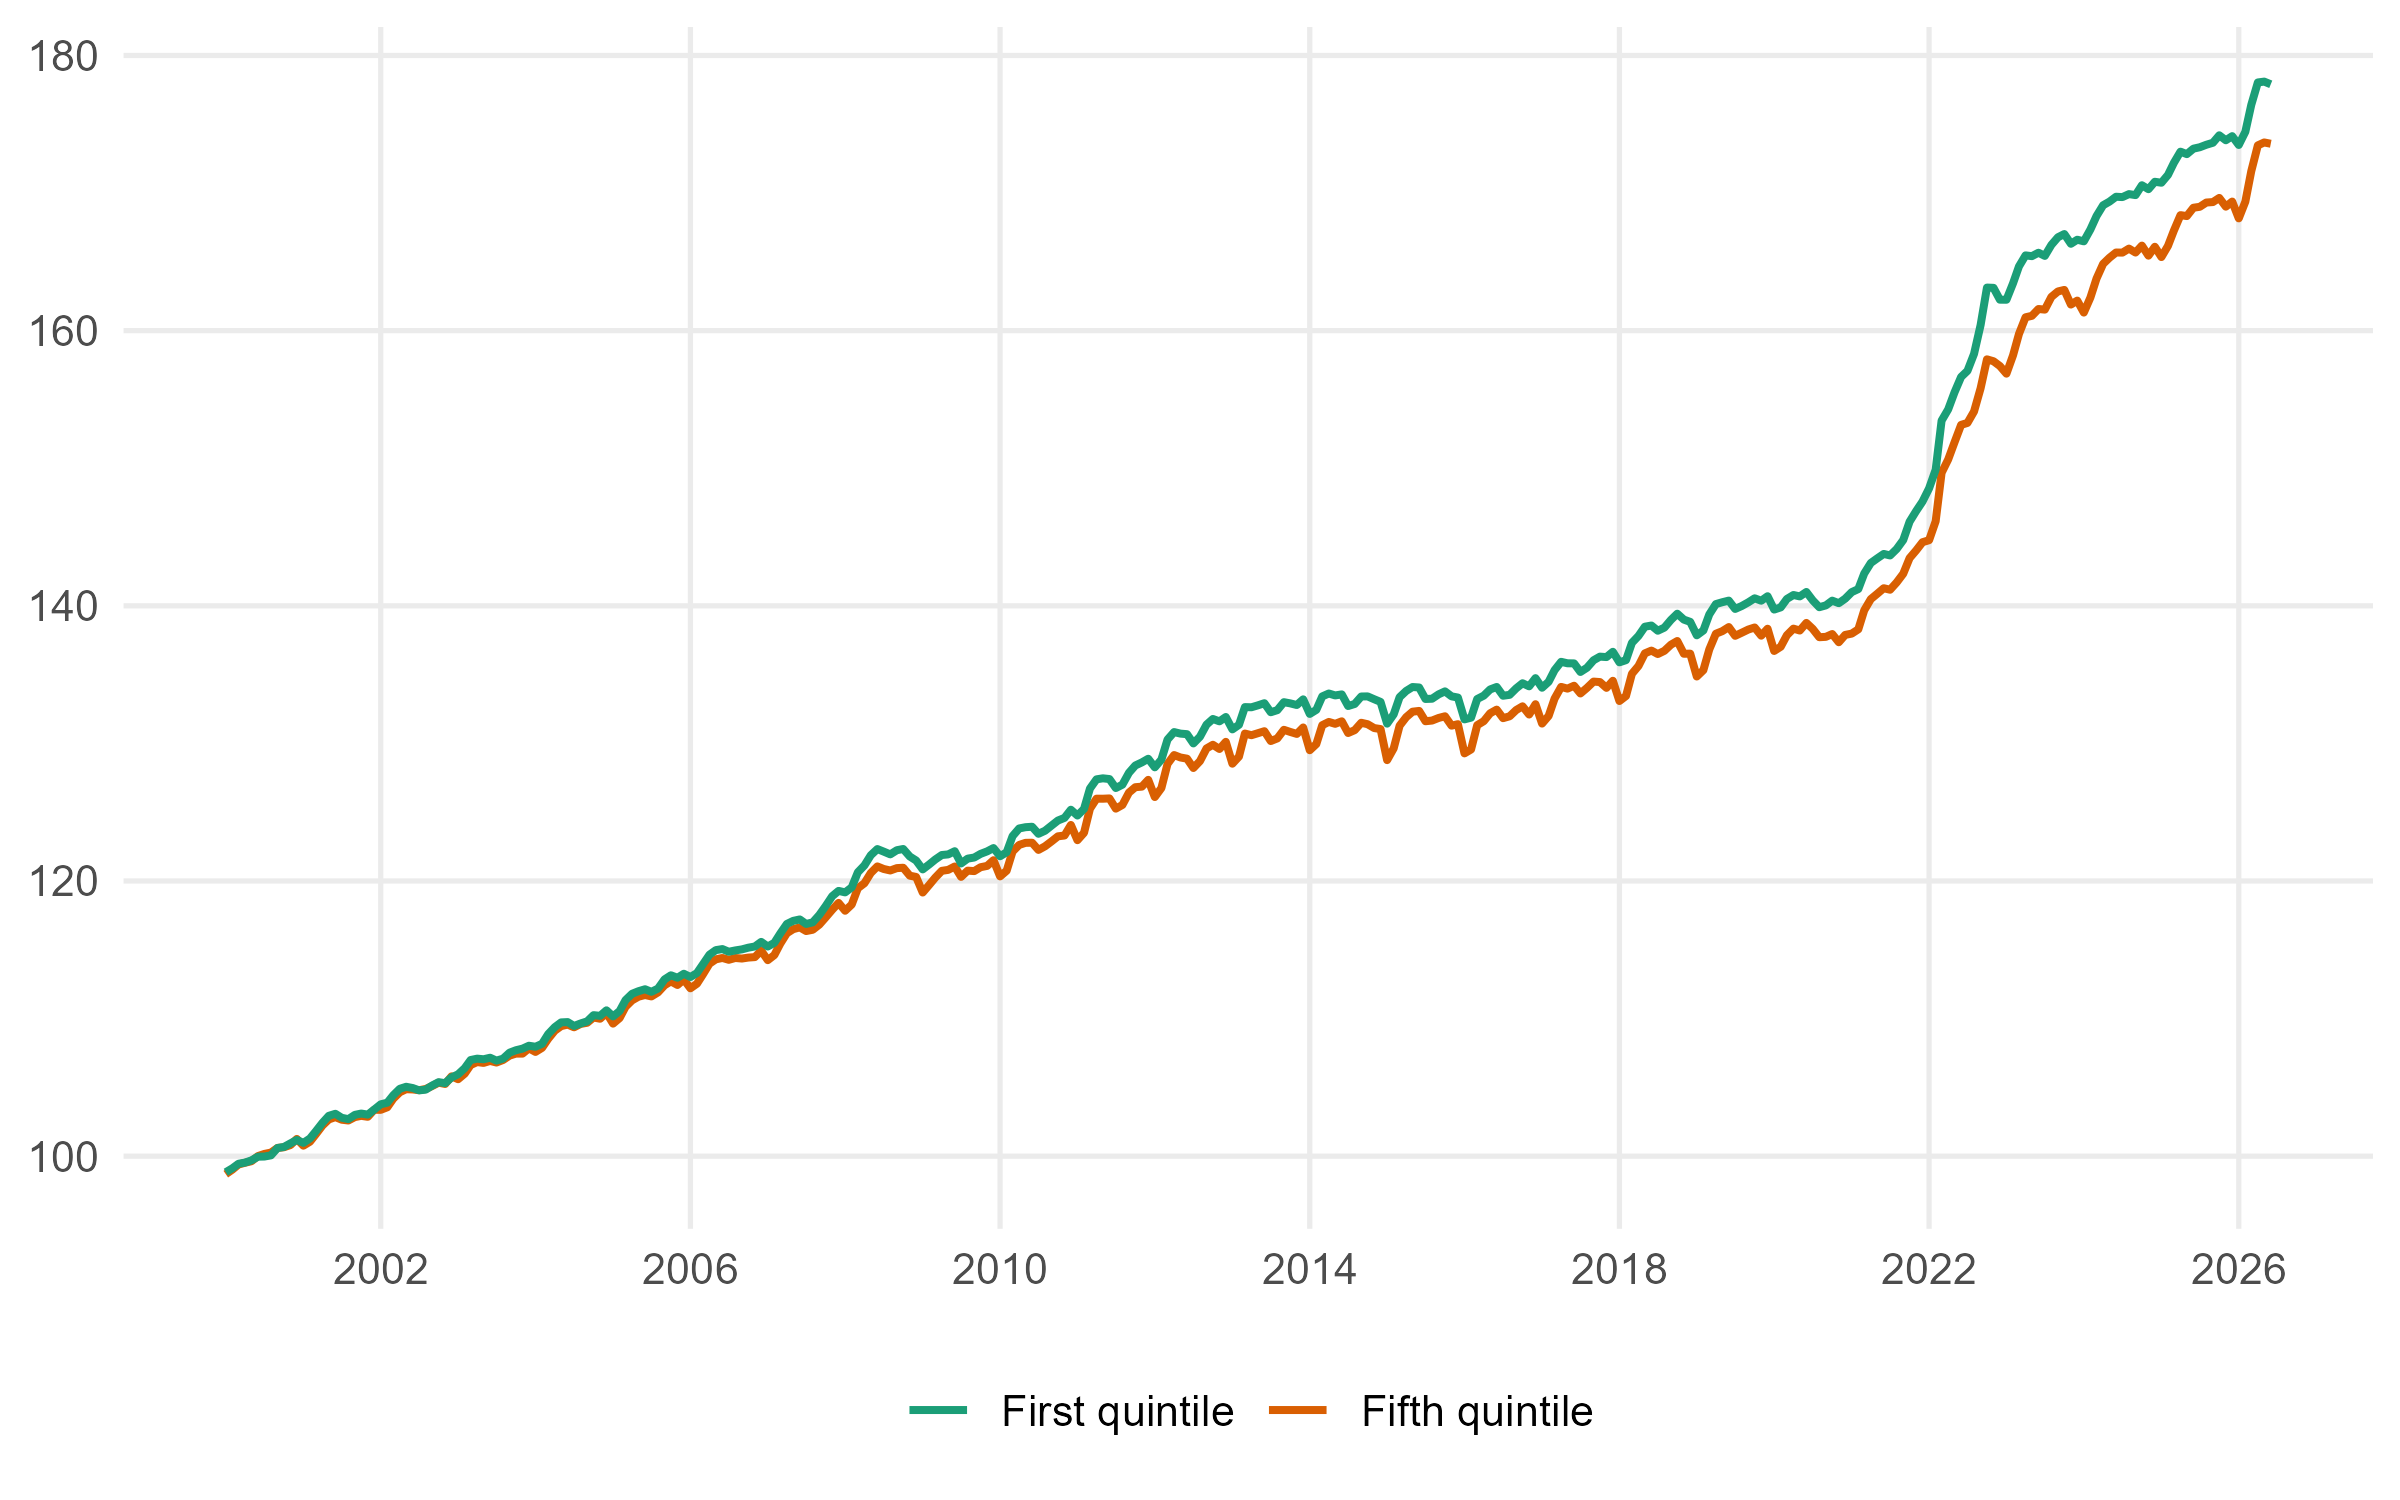
\includegraphics[width=0.82\textwidth,height=0.70\textheight,keepaspectratio]{fig/fig_EA20_2000_2026_income_price_index_Q1_Q5_base2000.png}
\source{Eurostat HICP and HBS; authors' calculations.}
\end{frame}

% 8
\begin{frame}{Cumulative Inflation Gap Across Countries, June 2021--June 2023}
\centering
\scriptsize
\begin{tabular}{lrrrr}
\toprule
Country & Total inflation & Q1 inflation & Q5 inflation & Gap\\
\midrule
Austria & 17.2 & 17.5 & 17.1 & 0.4\\
Cyprus & 12.0 & 12.7 & 12.0 & 0.7\\
Estonia & 33.0 & 38.7 & 31.2 & 7.5\\
Finland & 12.5 & 11.5 & 12.7 & -1.2\\
France & 12.2 & 12.3 & 12.1 & 0.2\\
Germany & 15.6 & 16.5 & 15.2 & 1.3\\
Ireland & 14.9 & 17.2 & 13.3 & 3.8\\
Italy & 15.8 & 17.2 & 15.1 & 2.1\\
Latvia & 28.9 & 36.0 & 26.5 & 9.5\\
Lithuania & 30.4 & 33.6 & 29.0 & 4.6\\
Netherlands & 16.9 & 17.7 & 16.5 & 1.2\\
Portugal & 14.2 & 13.1 & 15.4 & -2.3\\
Slovakia & 25.4 & 26.7 & 24.0 & 2.7\\
Spain & 11.8 & 11.8 & 11.7 & 0.1\\
\midrule
\textbf{Euro area} & \textbf{14.7} & \textbf{15.2} & \textbf{14.4} & \textbf{0.9}\\
\bottomrule
\end{tabular}
\source{Eurostat HICP and HBS; authors' calculations. Percentage points.}
\end{frame}

% 9
\begin{frame}{Product Contributions to the Income Inflation Gap}
\centering
\small
\begin{tabular}{lrrrr}
\toprule
Product group & Headline & Q1 & Q5 & Gap\\
\midrule
Food and non-alcoholic beverages & 4.3 & 5.2 & 4.5 & 0.7\\
Alcohol, tobacco and narcotics & 0.5 & 0.7 & 0.4 & 0.2\\
Clothing and footwear & 0.3 & 0.3 & 0.4 & -0.1\\
Housing, rentals and repairs & 1.2 & 0.4 & 0.6 & -0.2\\
Water, electricity, gas and fuels & 1.5 & 6.9 & 5.3 & 1.5\\
Transport & 1.9 & 1.6 & 2.8 & -1.2\\
Other & 5.0 & 0.2 & 0.3 & -0.1\\
\midrule
\textbf{Total} & \textbf{14.7} & \textbf{15.2} & \textbf{14.4} & \textbf{0.9}\\
\bottomrule
\end{tabular}
\vspace{1em}
\begin{itemize}
  \item Energy and food increase the Q1--Q5 gap; transport exposure offsets much of it.
\end{itemize}
\source{Eurostat HICP and HBS; authors' calculations. Percentage points.}
\end{frame}

% 10
\begin{frame}{Direct and Indirect Exposure to an Oil and Gas Shock}
\centering
\scriptsize
\begin{tabular}{lrrrrrr}
\toprule
Country & Total & Direct & Indirect & Gap & Gap direct & Gap indirect\\
\midrule
Austria & 11.8 & 3.9 & 7.9 & -1.4 & -0.7 & -0.7\\
Belgium & 9.8 & 6.2 & 3.7 & -3.6 & -3.2 & -0.4\\
Germany & 7.4 & 4.4 & 3.0 & -1.8 & -1.6 & -0.2\\
Estonia & 12.2 & 6.6 & 5.6 & -4.8 & -3.8 & -1.0\\
Spain & 7.4 & 4.5 & 3.0 & -1.9 & -1.6 & -0.3\\
France & 9.3 & 4.5 & 4.7 & -2.8 & -1.9 & -0.9\\
Italy & 9.2 & 4.9 & 4.3 & -1.9 & -1.3 & -0.6\\
Latvia & 14.1 & 7.2 & 6.9 & -7.9 & -4.9 & -3.0\\
Netherlands & 6.4 & 4.3 & 2.0 & -1.4 & -1.3 & 0.0\\
Portugal & 8.8 & 3.7 & 5.2 & -4.3 & -2.1 & -2.2\\
Slovakia & 12.5 & 6.3 & 6.2 & -0.5 & -0.4 & -0.1\\
\midrule
\textbf{Euro area} & \textbf{8.4} & \textbf{4.6} & \textbf{3.8} & \textbf{-2.2} & \textbf{-1.7} & \textbf{-0.5}\\
\bottomrule
\end{tabular}
\vspace{0.7em}
\begin{itemize}
  \item Uniform 40\% shock; price propagation is computed as $\Delta p=(I-A')^{-1}s$.
\end{itemize}
\source{Eurostat HICP, HBS and FIGARO; authors' calculations.}
\end{frame}

% 11
\begin{frame}{Unconventional Household Price Policies}
\begin{itemize}
  \item Electricity and gas price caps or tariff shields limited the retail prices paid by households.
  \item Temporary VAT and excise-tax reductions lowered consumer energy prices.
  \item Cuts in regulated network charges reduced electricity and gas bills.
  \item Fuel rebates and regulated discounts reduced prices at the pump.
  \item The counterfactual removes these price-based interventions while retaining observed prices for unaffected products.
  \item Direct income transfers and measures targeted only at firms are excluded from the price counterfactual.
  \item Policy effects are measured as observed inflation minus estimated no-policy inflation.
\end{itemize}
\source{National policy sources, Sgaravatti et al.; authors' calculations.}
\end{frame}

% 12
\begin{frame}{Household Price Policies and Average Inflation}
\centering
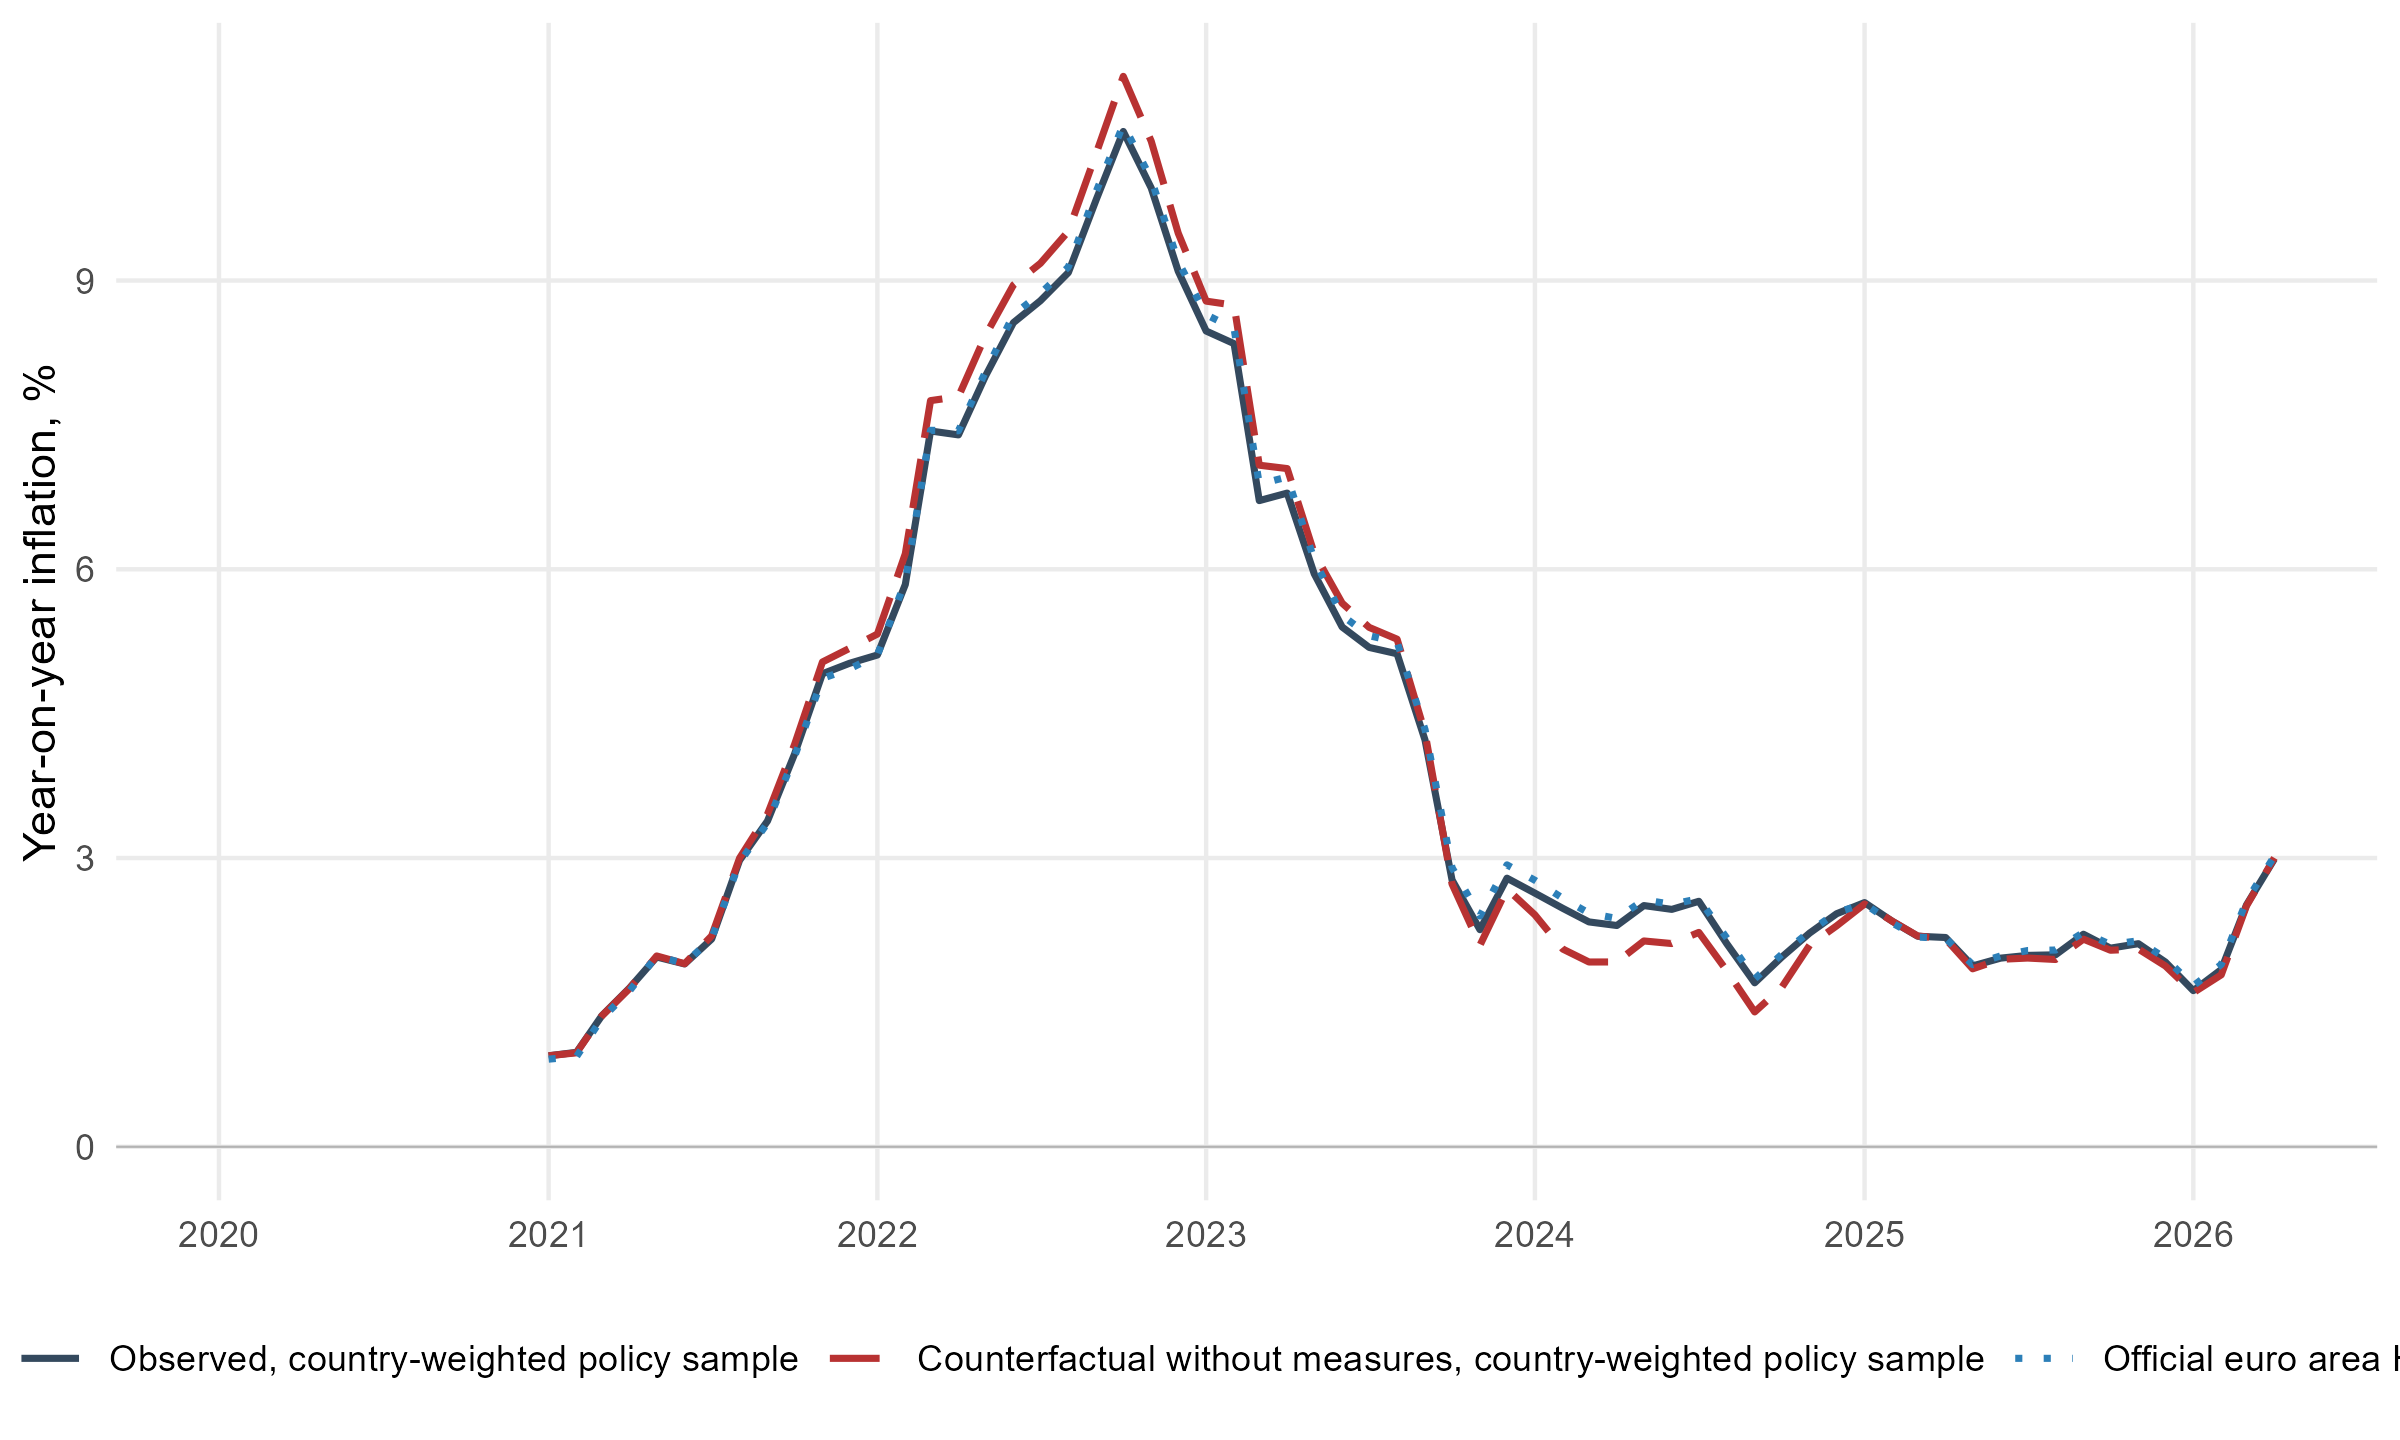
\includegraphics[width=0.82\textwidth,height=0.70\textheight,keepaspectratio]{fig/policy_total_cpi_counterfactual_inflation_EA_policy_sample.png}
\source{Eurostat and national statistical institutes; authors' calculations.}
\end{frame}

% 12
\begin{frame}{Household Price Policies and Inflation Inequality}
\centering
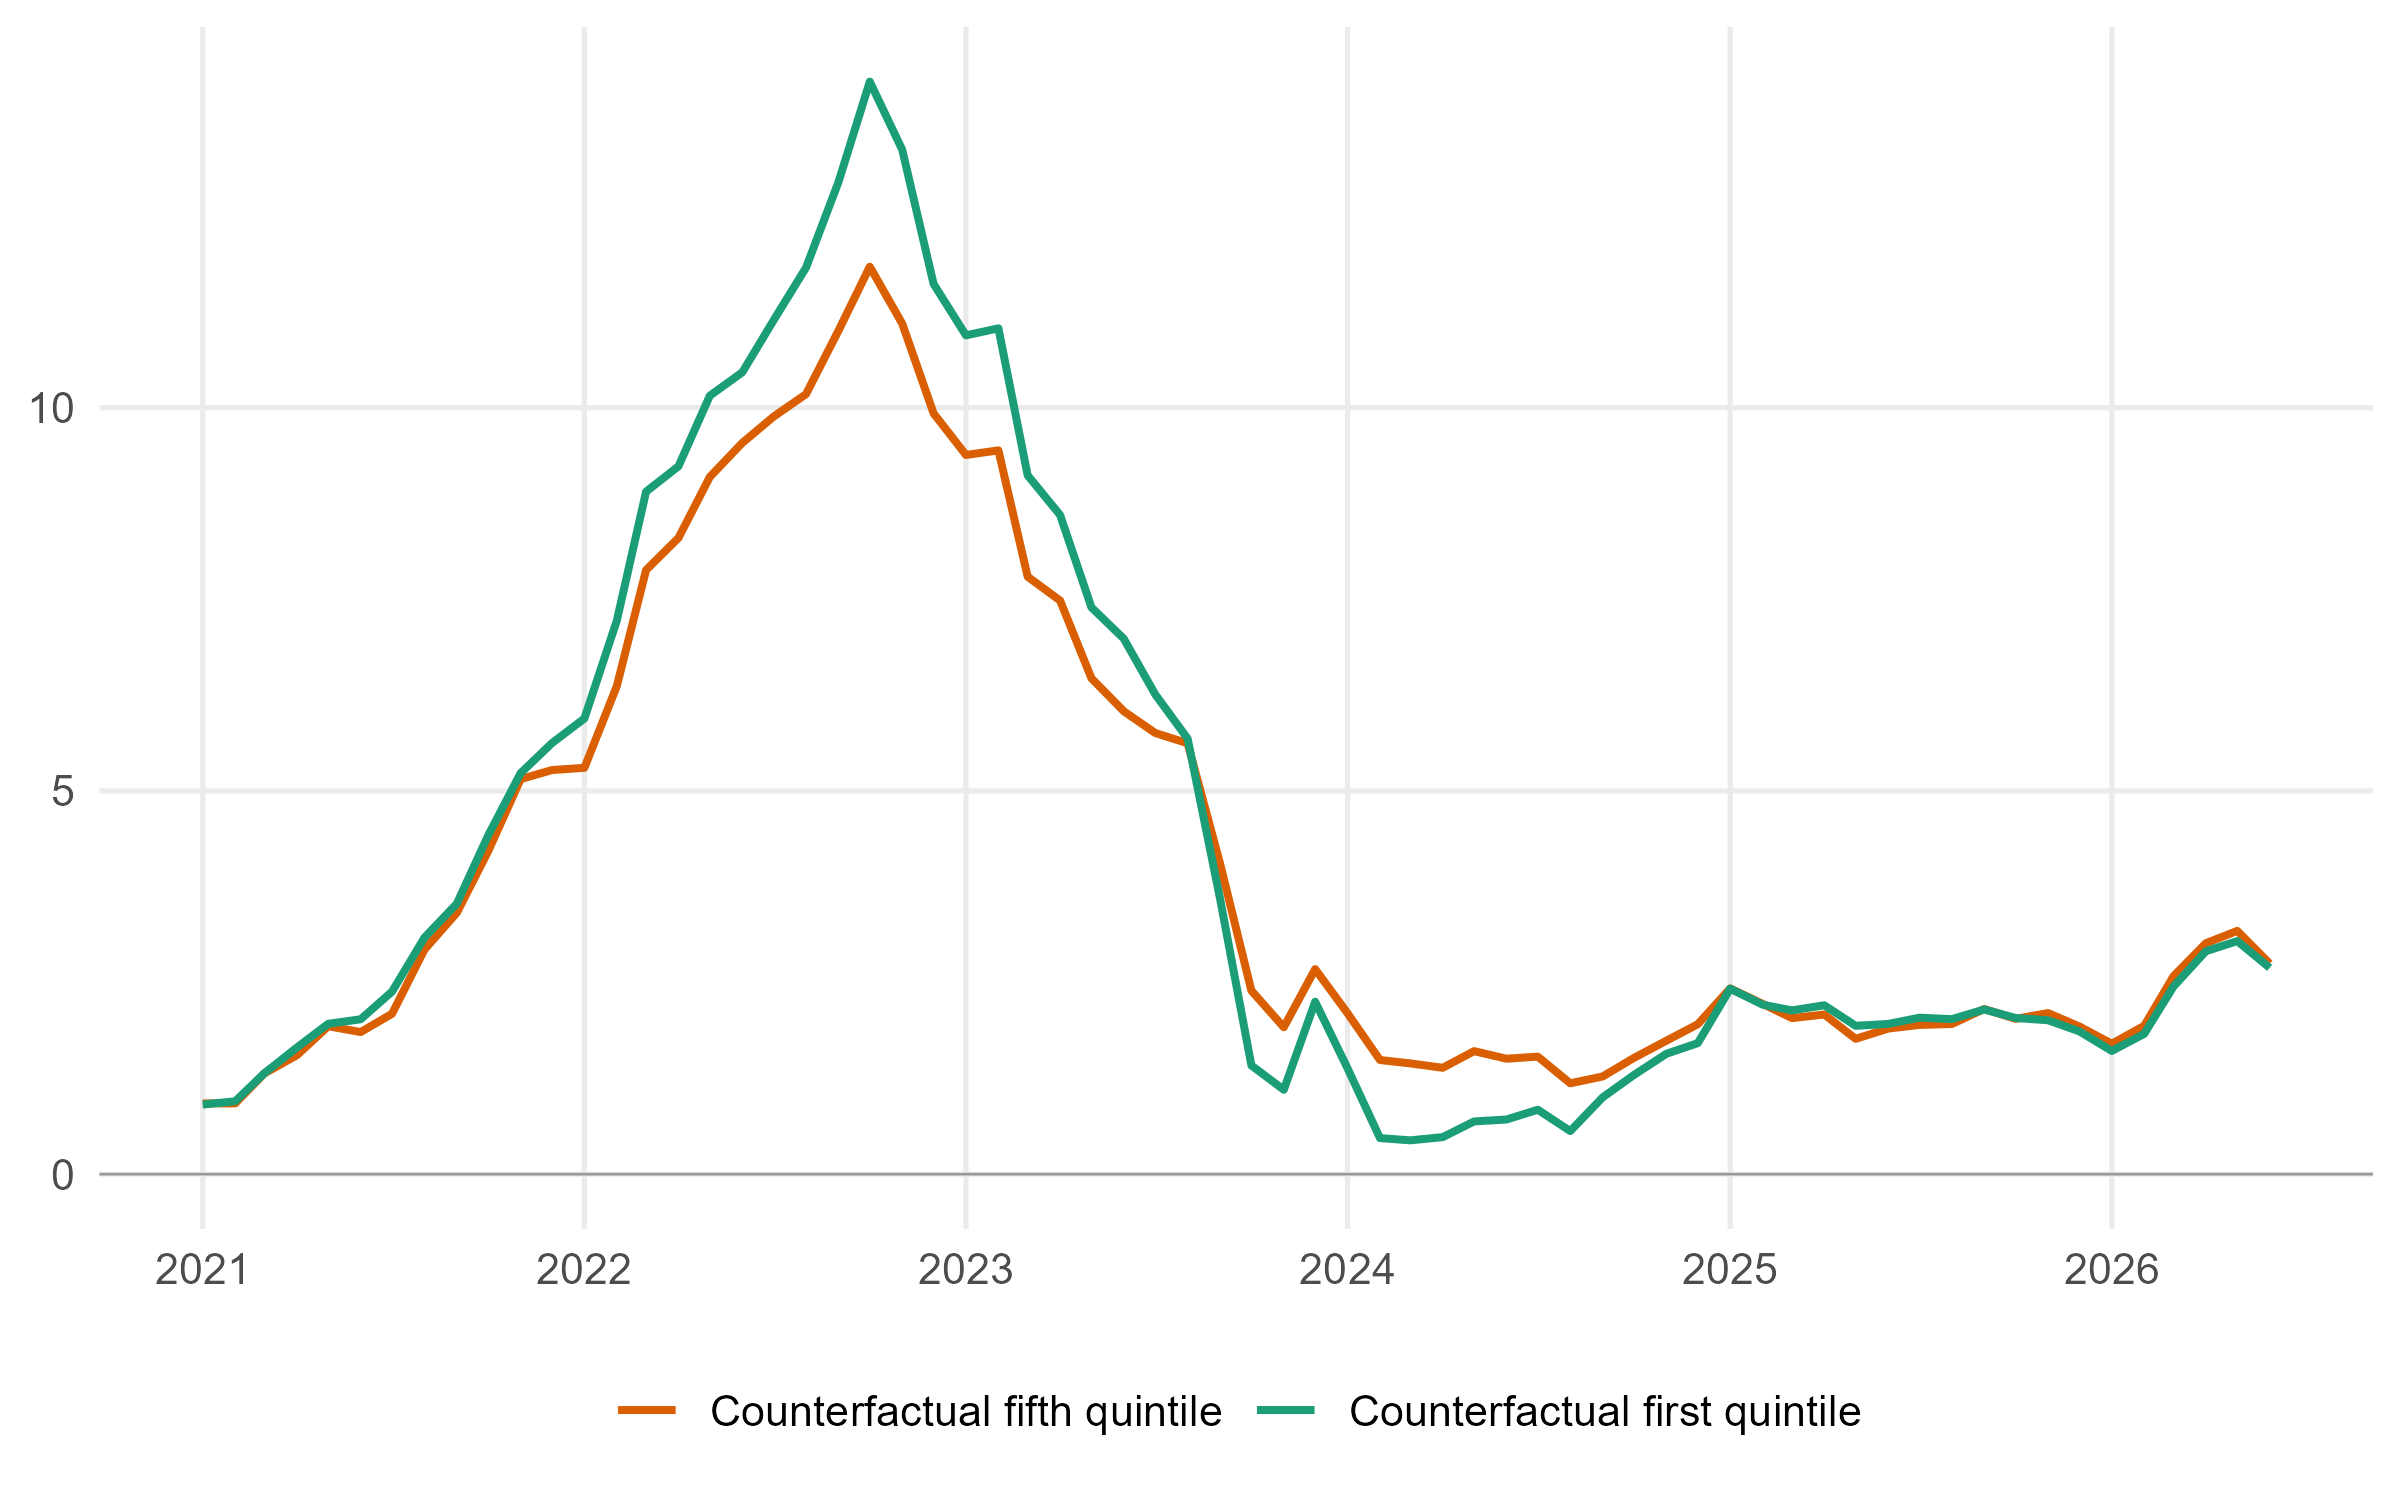
\includegraphics[width=0.82\textwidth,height=0.70\textheight,keepaspectratio]{fig/fig_EA20_2021_2026_counterfactual_income_inflation_Q1_Q5.png}
\source{Eurostat and national statistical institutes; authors' calculations.}
\end{frame}

% 13
\begin{frame}{Fiscal Cost and No-Policy Inflation Across Countries}
\centering
\scriptsize
\begin{tabular}{lrrrrrrr}
\toprule
Country & Cost & No-policy & Avg. effect & Q1 & Q5 & Gap & Gap effect\\
\midrule
Austria & 3.8 & 17.7 & -0.5 & 19.3 & 18.2 & 1.1 & -0.7\\
Estonia & 0.2 & 33.1 & -0.1 & 39.0 & 31.4 & 7.6 & -0.1\\
France & 80.5 & 14.0 & -1.8 & 19.4 & 16.6 & 2.8 & -2.6\\
Germany & 60.2 & 16.0 & -0.4 & 18.4 & 16.2 & 2.2 & -0.9\\
Ireland & 1.4 & 15.0 & -0.1 & 17.6 & 13.6 & 4.1 & -0.2\\
Italy & 36.2 & 16.1 & -0.3 & 18.2 & 15.8 & 2.4 & -0.3\\
Latvia & 0.7 & 29.2 & -0.2 & 37.2 & 27.0 & 10.2 & -0.6\\
Netherlands & 34.8 & 17.6 & -0.7 & 20.3 & 18.0 & 2.3 & -1.1\\
Portugal & 5.6 & 14.8 & -0.6 & 15.5 & 17.0 & -1.5 & -0.8\\
Slovakia & 2.3 & 26.9 & -1.6 & 33.5 & 27.8 & 5.7 & -3.0\\
Spain & 23.1 & 12.5 & -0.7 & 14.6 & 13.5 & 1.1 & -1.0\\
\midrule
\textbf{Euro area} & \textbf{266.9} & \textbf{15.4} & \textbf{-0.7} & \textbf{18.2} & \textbf{16.2} & \textbf{2.0} & \textbf{-1.2}\\
\bottomrule
\end{tabular}
\vspace{0.7em}
\begin{itemize}
  \item Negative effects indicate that price policies reduced inflation or the Q1--Q5 gap.
\end{itemize}
\source{Eurostat and national statistical institutes; authors' calculations.}
\end{frame}

% 14
\begin{frame}{Product-Level Effects of Household Price Policies}
\centering
\small
\begin{tabular}{lrrrrr}
\toprule
Product group & No-policy & Q1 & Q5 & Gap & Policy effect\\
\midrule
Food and non-alcoholic beverages & 4.5 & 5.4 & 4.6 & 0.8 & -0.1\\
Alcohol, tobacco and narcotics & 0.5 & 0.7 & 0.4 & 0.2 & 0.0\\
Clothing and footwear & 0.3 & 0.3 & 0.4 & -0.2 & 0.0\\
Housing, rentals and repairs & 0.5 & 0.4 & 0.6 & -0.2 & 0.0\\
Water, electricity, gas and fuels & 6.9 & 9.4 & 6.5 & 2.9 & -1.4\\
Transport & 2.4 & 1.8 & 3.2 & -1.4 & 0.2\\
Other & 0.3 & 0.2 & 0.4 & -0.2 & 0.0\\
\midrule
\textbf{Total} & \textbf{15.4} & \textbf{18.2} & \textbf{16.2} & \textbf{2.0} & \textbf{-1.2}\\
\bottomrule
\end{tabular}
\vspace{1em}
\begin{itemize}
  \item Energy accounts for almost all of the reduction in inflation inequality.
\end{itemize}
\source{Eurostat and national statistical institutes; authors' calculations.}
\end{frame}

% 15
\begin{frame}{Household-Level Inflation Burden}
\centering
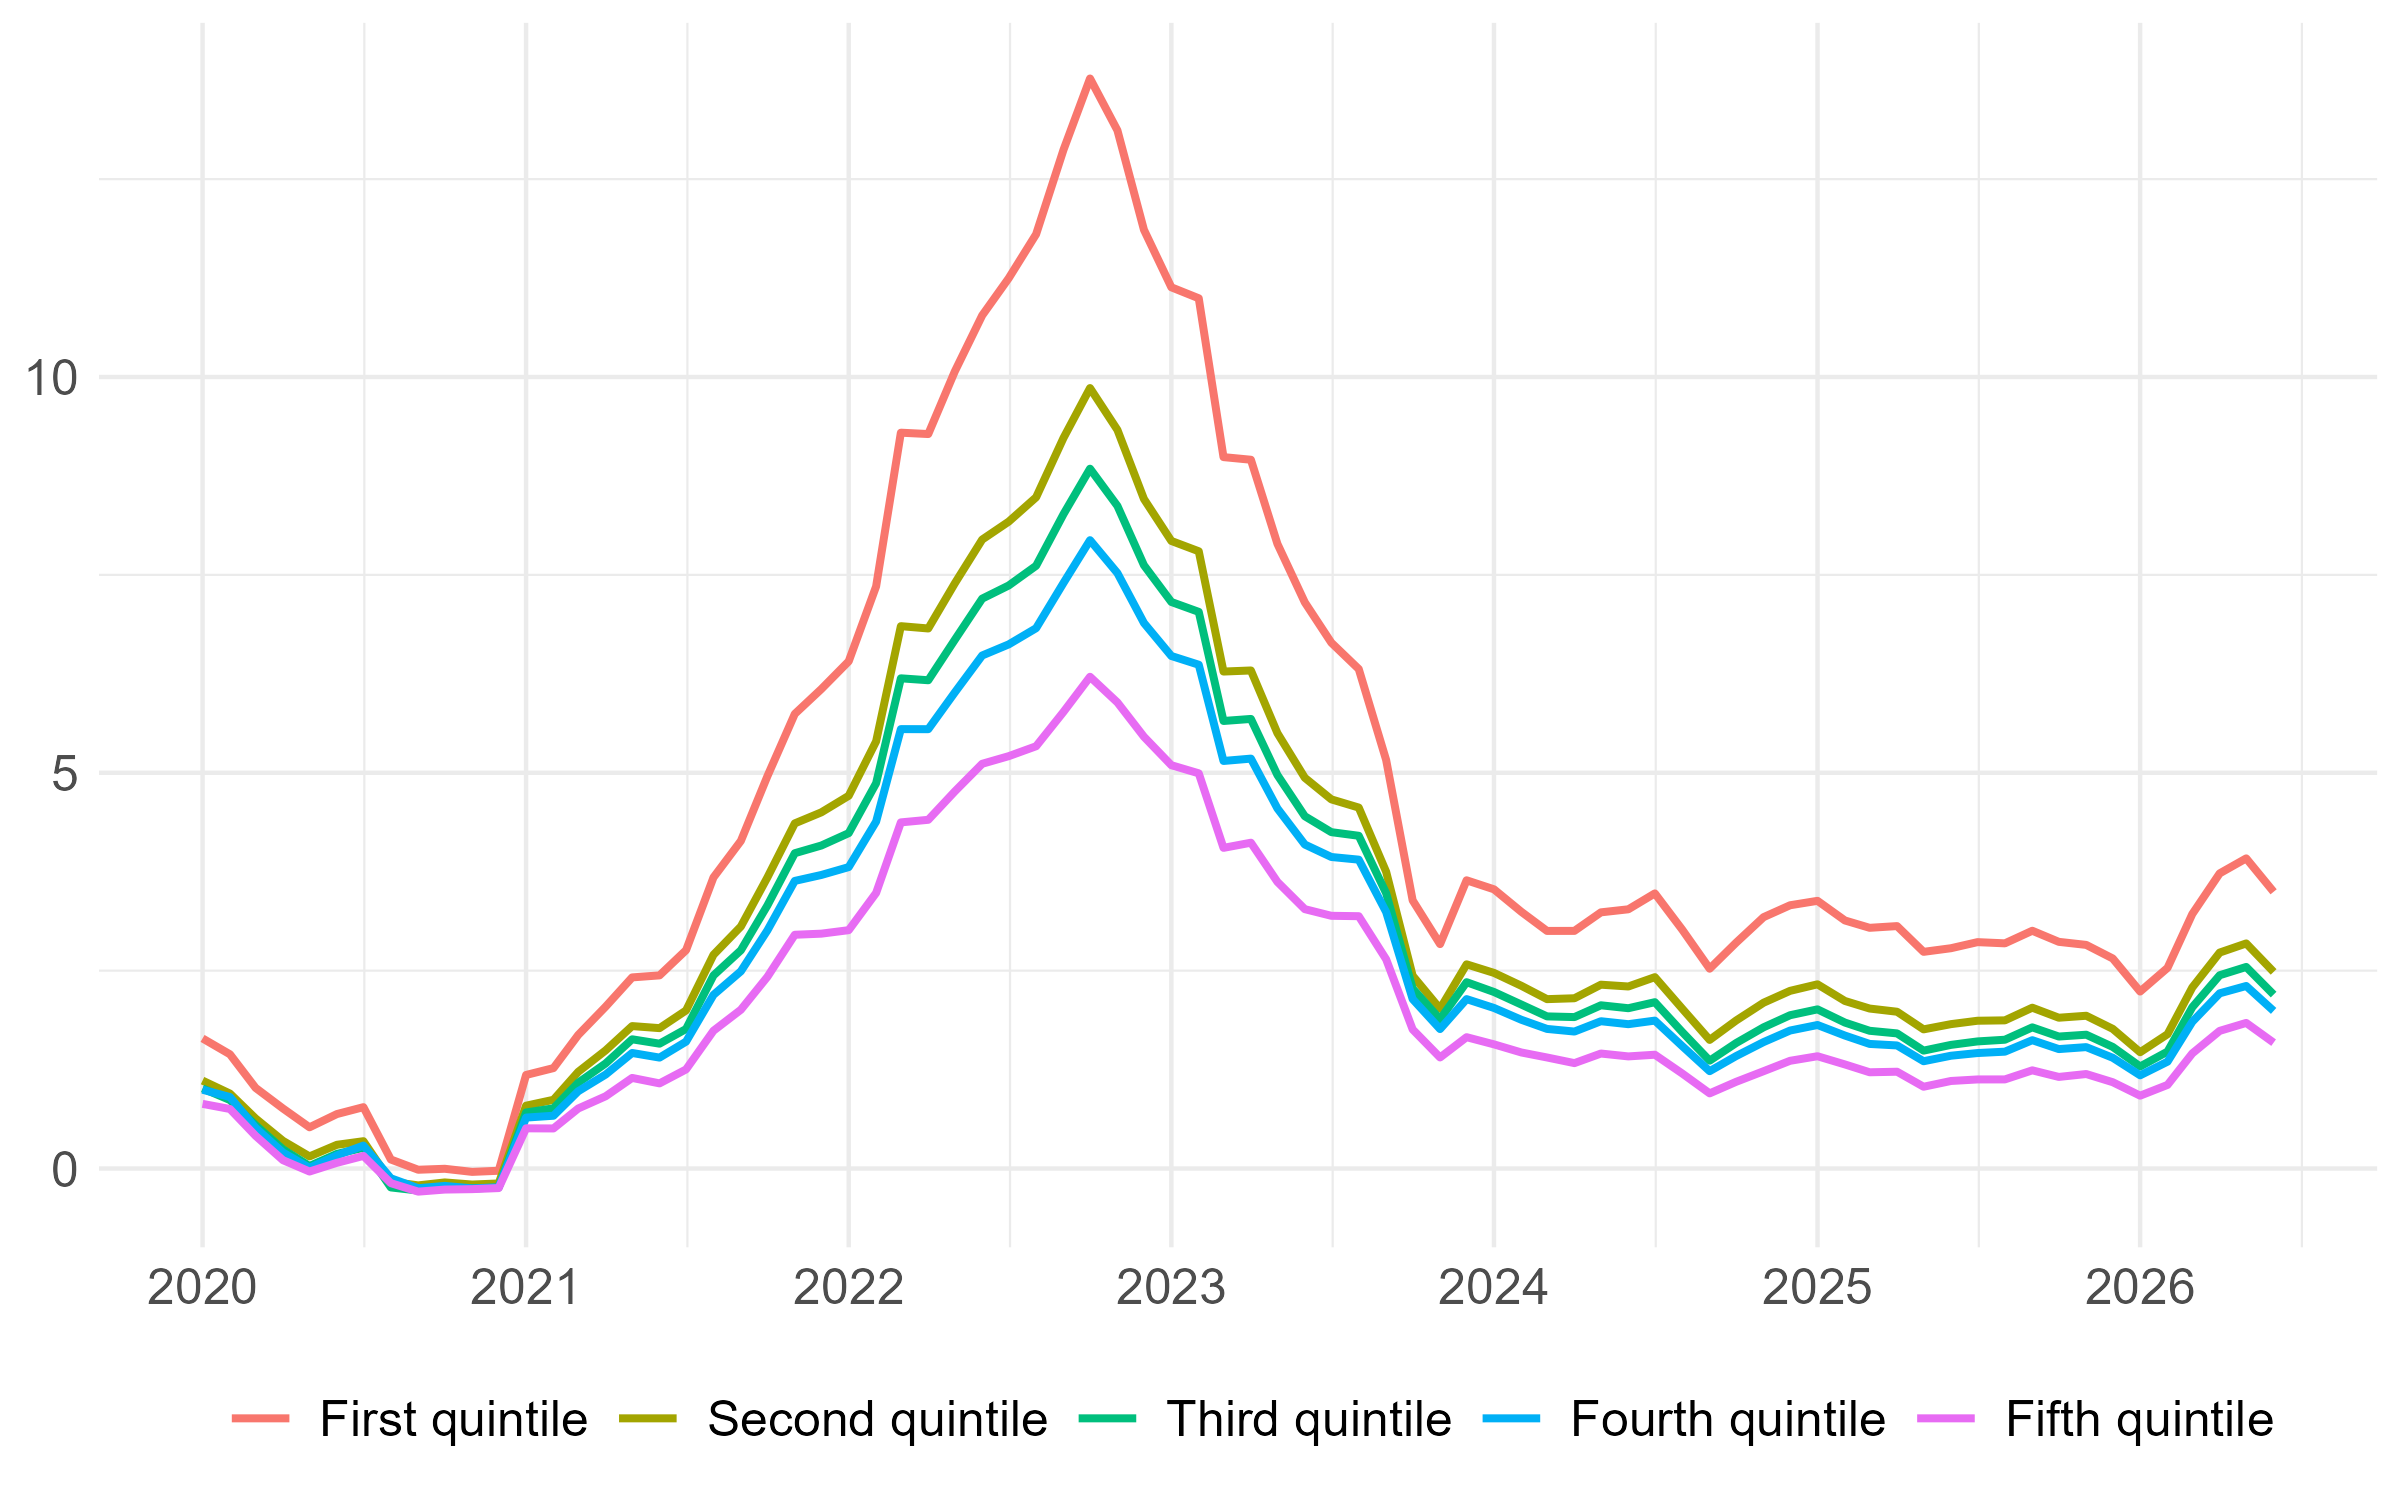
\includegraphics[width=0.70\textwidth,height=0.58\textheight,keepaspectratio]{fig/fig_EA20_2019_2026_income_inflation_burden_Q1_Q5.png}
\begin{itemize}
  \item Low-income households face a larger inflation burden relative to net income.
  \item Price policies reduced both average inflation and the income inflation gap.
\end{itemize}
\source{Eurostat HICP and HBS microdata; authors' calculations.}
\end{frame}

% 16
\begin{frame}{Conclusion}
\begin{itemize}
  \item Inflation differences between income groups are moderate for the euro area as a whole, but vary substantially across countries.
  \item Age and residence-area gaps were larger than the aggregate Q1--Q5 gap during the 2021--2023 inflation episode.
  \item Food and household energy increased inflation exposure for low-income households, while transport partly offset the income gap.
  \item Production networks transmitted energy shocks indirectly across sectors and countries.
  \item Household price policies lowered cumulative average inflation and reduced the Q1--Q5 inflation gap.
  \item Inflation remained more burdensome for low-income households because consumption represents a larger share of their net income.
\end{itemize}
\end{frame}

\end{document}
